% Author: Dun-Ming Huang
% Email: dunmingbrandonhuang@berkeley.edu
% CSM16A Fall 2022
\qns{Trying to Figure Out Flow of Department Funding}

\textbf{Learning Goal: }
\begin{bindenum}
    \item Learn what is a state transition system in matrix, diagram expressions
    \item Learn to identify and understand conservative and drained state transition systems.
\end{bindenum}

\meta{
    \begin{itemize}
        \item This is an \textbf{introduction towards state-transition matrix} before its eigen-analysis aspects of it, so we can present more challenging contents for eigenvalue-state transition on the coming weeks.
        \item Amidst problem-solving and teaching, please \textbf{clearly define} terms relating to state transition matrix (\textbf{\textit{conservative, draining, timestamp}}).
        \item This question \textbf{can be used during the walkthrough of state-transition matrices}, and \textbf{may be incorporated into your mini-lecture}. This question also attempts to review basic matrix mechanical calculations, such as inverse matrices and matrix-vector multiplication.
    \end{itemize}
}

You have been found by the Chancellor of University of Currying Brocolli, where you were provided a chart of financial details on this school's EEKS Department. Provided some financial data, and having learned about state-transition matrices, help the university's council on the following subtasks, and decide the fate of their funding!
\par
The money of EEKS Department flows between three locations: Courses (C), Dog Food (D), and Electrical engineering components (E).

\begin{enumerate}
    \item{
        Create a state transition matrix where, across any timestamp (from $t = k$ to $t = k + 1$), $50\%$ of funding for Courses is transferred to Dog Food, $80\%$ of funding from Electrical Engineering is transferred to Dog Food, and all funding that were allocated to Dog Food is now transferred to Courses.
    
    }
    \meta{
        Mentors can \textbf{use the table setup in the solution to explain the way state-transition matrices work}. \\
        This question is intended as an introduction towards state transition system, which may be used during the in-section mini-lecture for demonstration to \textbf{introduce the concept of timestamps, state transition, and states}.

    }
    \ans{
        We may organize the above information into a table first:
        \begin{center}
            \begin{tabular}{|c|c|c|c|}
                \hline
                $\downarrow$ To $\big|$ From $\rightarrow$ & Courses & Dog Food & Electrical Engineering \\
                \hline
                Courses & $0\%$ & $100\%$ & $0\%$ \\
                \hline
                Dog Food & $50\%$ & $0\%$ & $80\%$ \\
                \hline
                Electrical Engineering & $0\%$ & $0\%$ & $0\%$ \\
                \hline
            \end{tabular}
        \end{center}
        which the format corresponds strikingly similar to the way state transition matrices are formulated in, expressed as follows:
        \[
            A = 
            \begin{bmatrix}
                0 & 1 & 0 \\
                0.5 & 0 & 0.8 \\
                0 & 0 & 0 \\
            \end{bmatrix}
        \]
        The state diagram would then be drawn as:
        % Author: Dun-Ming Huang
% Email: dunmingbrandonhuang@berkeley.edu
% CSM16A Fall 2022
% Code for operational amplifier and comparator comes from q_comparators.tex of CSM16A

\begin{circuitikz}
    \draw (0,0) node[op amp,yscale=-1] (opamp) { }
      (opamp.out) node[right ] {$V_{out}$} 
      ;
	\draw (-0.2, -0.2) to [short] (0, -0.2) to [short] (0, 0.2) to [short] (0.2, 0.2);
    \draw
        (0, 0.5)
            to [short] (0, 1.0)
            to [V, l^=$5V$] (2, 1) node[ground]{}
        ;
    \node[draw=none,text=black] at (0, 2) {$V_{DD}$};
    \draw (0, -0.5) to [short] (0, -1.0) node[ground]{};
    \node[draw=none,text=black] at (0, -2) {$V_{SS}$};
    
    \draw[draw=black] (-11, 0) rectangle (-8, 1);
    \node[] at (-9.5, 0.5) {Sound Sensor};
    
    \draw (-8, 0.5) to [short] (-7.5, 0.5);
    
    \draw[draw=black] (-7.5, 0) rectangle (-3.5, 1);
    \node[] at (-5.5, 0.5) {Sound-Volt Converter};
    
    \draw
        (-3.5, 0.5)
            to [short] (opamp.+)
        (-3.5, -0.5) node[ground]{}
            to [V, invert, l_=$3V$] (opamp.-)
        ;
\end{circuitikz}

    }

    \item{
        Translate the following state diagram into a state transition matrix:
        \begin{center}
    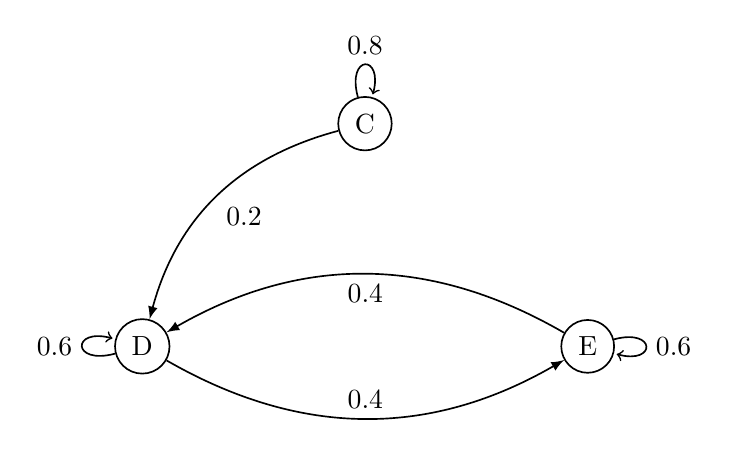
\begin{tikzpicture}[-latex, auto, node distance={4cm}, semithick, main/.style = {draw, circle}]
        \node[main] (C) {C};
        \node[main, below left of = C] (D) {D};
        \node[main, below right of = C] (E) {E};
        \path (C) edge[loop above] node{0.8} (C);
        \path (C) edge[bend right] node{0.2} (D);
        \path (D) edge[loop left] node{0.6} (D);
        \path (D) edge[bend right] node{0.4} (E);
        \path (E) edge[bend right] node{0.4} (D);
        \path (E) edge[loop right] node{0.6} (E);
    \end{tikzpicture}
\end{center}


    
    }
    \meta{
        The intention and suggested usage of this question subpart is as written for subpart (a).

    }
    \ans{
        We may organize the above information into a table first:
        \begin{center}
            \begin{tabular}{|c|c|c|c|}
                \hline
                $\downarrow$ To $\big|$ From $\rightarrow$ & Courses & Dog Food & Electrical Engineering \\
                \hline
                Courses & $0.8$ & $0$ & $0$ \\
                \hline
                Dog Food & $0.2$ & $0.6$ & $0.4$ \\
                \hline
                Electrical Engineering & $0$ & $0.4$ & $0.6$ \\
                \hline
            \end{tabular}
        \end{center}
        which the format corresponds strikingly similar to the way state transition matrices are formulated in, expressed as follows:
        \[
            A = 
            \begin{bmatrix}
                0.8 & 0 & 0 \\
                0.2 & 0.6 & 0.4 \\
                0 & 0.4 & 0.6 \\
            \end{bmatrix}
        \]

    }

    \item{
        Provided the following state diagram from part (b), provided that the total amount of funding at timestamp $k$ is $M$, and the representing vector of funding across aspects of departments is $\vec{m}[k]$, what is the total amount of funding at timestamp $k + 100$?
    
    }
    \meta{
        This subpart is \textbf{intended to introduce conservative state transition systems}. \\
        Instructors may choose to:
        \begin{itemize}
            \item Define ``conservative'', and use this question to demonstrate
            \item Use as a subpart for students to give feedback on, and then discuss ``conservative''
        \end{itemize}
        The subpart isn't introducing a definition for conservative systems yet in the case lectures end up not covering it. Therefore, \textbf{this is just an observation-based} subpart. \\
        Meanwhile, make sure to \textbf{lead students to understand the last statement of this solution, as it requires some mathematical explanation}. Hopefully, this brings a deepened understanding to the conservativeness of conservative systems (consistency of content quantity in a system).

    }
    \ans{
        Let us express the components of funding as follows:
        \[
            \begin{cases}
                m_c[t] = &\text{ Funding that Courses hold at timestamp $t$} \\
                m_d[t] = &\text{ Funding that Dog Food hold at timestamp $t$} \\
                m_e[t] = &\text{ Funding that Electrical Engineering hold at timestamp $t$} \\
            \end{cases}
        \]
        Let us first observe what happens to the total amount of funding after one timestamp:
        \begin{align*}
            M_{t = k + 1}
            &= sum(A \vec{m}[k]) \\
            &= sum \bigg(
            \begin{bmatrix}
                0.8 & 0 & 0 \\
                0.2 & 0.6 & 0.4 \\
                0 & 0.4 & 0.6 \\
            \end{bmatrix}
            \begin{bmatrix}
                m_c[k] \\ m_d[k] \\ m_e[k]
            \end{bmatrix} \bigg) \\
            &= (0.8 m_c[k]) + (0.2 m_c[k] + 0.6 m_d[k] + 0.4 m_e[k]) + (0.4 m_d[k] + 0.6 m_e[k]) \\
            &= m_c[k] + m_d[k] + m_e[k] = sum(\vec{m}[k]) = M_{t = k}
        \end{align*}
        Therefore, no matter how many timestamps have passed, the total amount of funding in this system will remain the same. \\
        Essentially,
        \[
            M_{t = k} = M_{t = k + 1} = M_{t = k + 2} = \cdots = M_{t = k + 100}
        \]

    }

    
    \item{
        Along the state transition system in part (b), the chancellor provides you a data about funding on each aspect of the department (courses, dog food, electrical components) at timestamp $n$ to be:
        \[
            \vec{v}[n] = \begin{bmatrix} 32 \\ 128 \\ 112 \end{bmatrix}
        \]
        What would be the funding of each department at timestamp $n - 2$?
    
    }
    \meta{
        This question demands students to first find a method to access data about previous timestamp, and then perform computations to access data from previous timestamps. \textbf{Useful hints can be ``how do we divide a matrix from one side of some equation''}. \\
        This might make a \textbf{good opportunity to have students collaboratively walkthrough a subpart} to get to talk with their new classmates, provided this subpart is indeed a multi-part problem by itself.

    }
    \ans{
        \textbf{General Approach:}\\
        Provided the general relationship that:
        \[
            \vec{v}[n + 1] = A \vec{v}[n]
        \]
        assuming $A$ is invertible, then we may suppose the relationship that:
        \[
            A^{-1} \vec{v}[n + 1] = \vec{v}[n]
        \]
        Therefore, if we can find the inverse of $A$, we can use the above relationship to deduce the value of $\vec{v}[n - 2]$.
        \par
        \textbf{Finding the Inverse of $A$:}\\
        Let us find the inverse of $A$ using Gauss Jordan Elimination:
        \begin{align*}
            \begin{sysmatrix}{rrr|rrr}
                0.8 & 0 & 0 & 1 & 0 & 0 \\
                0.2 & 0.6 & 0.4 & 0 & 1 & 0 \\
                0 & 0.4 & 0.6 & 0 & 0 & 1
            \end{sysmatrix}
            &\ro{R_2 \rightarrow 4R_2 - R_1}
            \begin{sysmatrix}{rrr|rrr}
                0.8 & 0 & 0 & 1 & 0 & 0 \\
                0 & 2.4 & 1.6 & -1 & 4 & 0 \\
                0 & 0.4 & 0.6 & 0 & 0 & 1
            \end{sysmatrix} \\
            &\ro{R_3 \rightarrow 6R_3 - R_2}
            \begin{sysmatrix}{rrr|rrr}
                0.8 & 0 & 0 & 1 & 0 & 0 \\
                0 & 2.4 & 1.6 & -1 & 4 & 0 \\
                0 & 0 & 2 & 1 & -4 & 6
            \end{sysmatrix} \\
            &\ro{R_2 \rightarrow \frac{5}{4}R_2 - R_3}
            \begin{sysmatrix}{rrr|rrr}
                0.8 & 0 & 0 & 1 & 0 & 0 \\
                0 & 3 & 0 & -\frac{9}{4} & 9 & -6 \\
                0 & 0 & 2 & 1 & -4 & 6
            \end{sysmatrix} \\
            &\ro{\text{Settling up on rows}}
            \begin{sysmatrix}{rrr|rrr}
                1 & 0 & 0 & \frac{5}{4} & 0 & 0 \\
                0 & 1 & 0 & -\frac{3}{4} & 3 & -2 \\
                0 & 0 & 1 & \frac{1}{2} & -2 & 3
            \end{sysmatrix}
        \end{align*}
        We have then obtained the result,
        \[
            A^{-1} = 
            \begin{bmatrix}
                \frac{5}{4} & 0 & 0 \\
                -\frac{3}{4} & 3 & -2 \\
                \frac{1}{2} & -2 & 3
            \end{bmatrix}
        \]
        and may verify it upon multiplying with $A$ and observe whether its product is the identity matrix.
        \par
        \textbf{Computing for $\vec{v}[n - 2]$:} \\
        Having found $A^{-1}$, let us consider the following computation:
        \begin{align*}
            \vec{v}[n - 1] &= A^{-1} \vec{v}[n] \\
            \vec{v}[n - 2] &= A^{-1} A^{-1} \vec{v}[n] \\
            &=
            \begin{bmatrix}
                \frac{5}{4} & 0 & 0 \\
                -\frac{3}{4} & 3 & -2 \\
                \frac{1}{2} & -2 & 3
            \end{bmatrix}
            \begin{bmatrix}
                \frac{5}{4} & 0 & 0 \\
                -\frac{3}{4} & 3 & -2 \\
                \frac{1}{2} & -2 & 3
            \end{bmatrix}
            \begin{bmatrix}
                32 \\ 128 \\ 112
            \end{bmatrix} \\
            &=
            \begin{bmatrix}
                \frac{25}{16} & 0 & 0 \\
                -\frac{67}{16} & 13 & -12 \\
                \frac{29}{8} & -12 & 13
            \end{bmatrix}
            \begin{bmatrix}
                32 \\ 128 \\ 112
            \end{bmatrix}
            =
            \begin{bmatrix}
                50 \\ 186 \\ 36
            \end{bmatrix}
        \end{align*}

    }

    \item {
        Now, provided the following state diagram:
        \begin{center}
    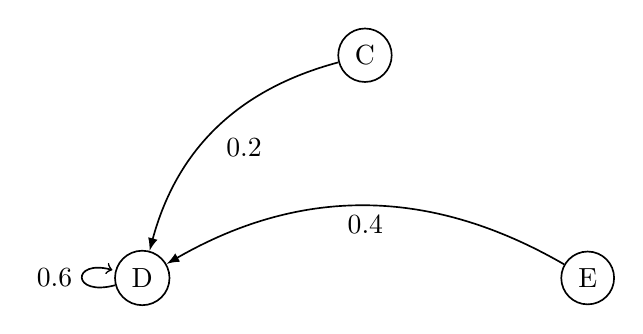
\begin{tikzpicture}[-latex, auto, node distance={4cm}, semithick, main/.style = {draw, circle}]
        \node[main] (C) {C};
        \node[main, below left of = C] (D) {D};
        \node[main, below right of = C] (E) {E};
        \path (C) edge[bend right] node{0.2} (D);
        \path (D) edge[loop left] node{0.6} (D);
        \path (E) edge[bend right] node{0.4} (D);
    \end{tikzpicture}
\end{center}
        the total amount of funding at timestamp $t$ is $N$, what occurs to the total amount of funding at timestamps beyond $t$? Furthermore, what would the total amount of funding be at an extremely long time (almost infinite) after timestamp $t$?
    
    }
    \meta{
        This is an \textbf{equivalent subpart of part (c) by intention, except now it explains a draining system}. This subpart is also not written to indirectly express concern on dog food funding. \\
        You can also \textbf{set up a jupyter notebook for the section} to see that the amount of content decreases throughout time:
        \begin{quote}
            Small tip for this: use np.array(), have a function for multiplying a state, and have a \textbf{print statement to summarize the growth of amount} over time. If you're really motivated, use \textbf{matplotlib to plot the decrease of total amount of contents} too!
        \end{quote}

    }
    \ans{
        Let us express the components of funding as follows:
        \[
            \begin{cases}
                n_c[t] = &\text{ Funding that Courses hold at timestamp $t$} \\
                n_d[t] = &\text{ Funding that Dog Food hold at timestamp $t$} \\
                n_e[t] = &\text{ Funding that Electrical Engineering hold at timestamp $t$} \\
            \end{cases}
        \]
        For each timestamp, the total amount of funding within the department reduces as described in the following:
        \begin{align*}
            N_k &= sum(\vec{n} [t = k]) = n_c[k] + n_d[k] + n_e[k] \\
            N_{k + 1} &= 0.2 n_c[k] + 0.6 n_d[k] + 0.4 n_e[k]
        \end{align*}
        eventually, across a really long time, the department's funding would be reduced to $0$ because there is a continuous drainage of money that does not cease.

    }
\end{enumerate}
